\documentclass{article}
\usepackage{color}
\usepackage{graphicx}
\usepackage[a4paper, hmargin=25mm, vmargin=30mm, top=20mm]{geometry}
\begin{document}
	\begin{center}
		\LARGE{\color{magenta}\textsc{\textbf{Bhumika Varshney}}
			\rule{\textwidth}{0.5mm}}
	\end{center}
	\begin{tabular}{l l}
		Near Munsif court, & \qquad\qquad\qquad\qquad\qquad\qquad Mob no: 9565844684 \\
		Main Road,Bisauli-202520 & \qquad\qquad\qquad\qquad\qquad\qquad Email id: bhumikavarshney4@gmail.com \\
		distt.-Budaun & \\
		Uttar Pradesh & \\
	\end{tabular}
	\begin{figure}[h]
		\begin{flushright}
			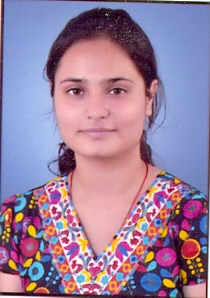
\includegraphics[scale=0.25]{bhumika.jpg}\\
		\end{flushright}		
	\end{figure}
	\\
	\underline{\textbf{OBJECTIVE}}- To obtain a position that will enable me to use my strong organizational skills, educational background, and ability to work well with people.
		\\
		\\
		\underline{\textbf{EDUCATION:}}\\
		\\
		\begin{tabular}{|p{3cm}|p{4cm}|p{3cm}|p{2cm}|p{3cm}|}
			\hline
			\textbf{Degree}& \textbf{College/school} & \textbf{University/Board} & \textbf{Passing Year} & \textbf{Pass Percentage} \\	
			\hline
			B.tech(currently in 4th semester) & JK Institute of Applied Physics and Technology & University of Allahabad & 2013-17 & 80\% (aggregate of $1^{st}$ and $2^{nd}$ semester)\\
			\hline
			Intermediate & Birla Balika Vidyapeeth, pilani & CBSE & 2013 & 96.8\% \\
			\hline
			High school & Birla Balika Vidyapeeth, pilani & CBSE & 2011 & 10 CGPA(95\%) \\
			\hline
		\end{tabular}
			\\
			\\
			\\
			\underline{\textbf{PROJECTS:}}\\
			\begin{enumerate}
				\item 
				\item
			\end{enumerate}
			\underline{\textbf{TRAINING \& SEMINARS ATTENDED:}}\\
			\\
			\begin{tabular}{|p{4.5cm}|p{4.5cm}|p{2cm}|p{4cm}|}
				\hline
				\textbf{Event} & \textbf{Institution} & \textbf{Year} & \textbf{Key Learning}\\
				\hline
				Seminar on youth leadershipin science at CEERI & Council of electronics and electrical research institute & 2012 & knowlwdge of basic space science \\
				\hline
				Attended SAARC  nations conference held in Sri Lanka & National Cadet Corps Sri Lanka & 2012 & Learned about emerging relationships among various countries \\
				\hline
				NCC training for 4 years & National Cadet Corps & 2009-12 & Unity and Discipline \\
				\hline
				Zonal seminar on ICT of IETE & J.K.Institute of applied physics and technology,Allahabad & 2014 & Communication Systems\\
				\hline
				Seminar on food technology by food minister of Rajasthan & Birla Balika Vidyapeeth & 2009 & Importance of good health \\
				\hline
			\end{tabular}
				\\
				\\
				\\
				\underline{\textbf{RESEARCH PUBLICATIONS:}}\\
				\begin{itemize}
					\item No research work done till yet.
						\\[\baselineskip]
				\end{itemize}
				\underline{\textbf{TECHNICAL SKILLS:}}\\
				\begin{enumerate}
					\item Robotics
					\item C programming
					\item Java programming
				\end{enumerate}
				\begin{center}
					\emph{\textbf{Secured 1st position in IIT BOMBAY, E-Yantra All India Robotics Competition 2014, Warehouse Management Theme}\\
						Awarded for developing a \textbf{fully autonomous Warehouse Managing robot} based on the Firebird V Platform, \textbf{amongst 33 teams all over India}, sponsored by Ministry of Human Resource Development (MHRD), Govt. of India.}
					\\[\baselineskip]
				\end{center}
				\underline{\textbf{SOFT SKILLS/ KEY STRENGTHS:}}\\
				\begin{enumerate}
					\item Effective communicator with excellent planning, organizational, and negotiation strengths as well as the ability to lead, read consensus, establish goals, and attain results.
					\item Good literacy and numeracy skills.
					\item Effective time management and be able to prioritise.
					\item Deterministic regarding work
					\item Optimistic attitude
					\\[\baselineskip]
				\end{enumerate}
				\underline{\textbf{EXTRA CURRICULAR ACTIVITIES:}}\\
				\begin{itemize}
					\item Class Prefect in class $10^{th}$
					\item \textbf{House Captain} of my house in school
					\item Trained \textbf{Kathak dancer}, 4 years training in this dance form
					\item Knowledge of many folk dances like Rajasthani, Gujarati, Punjabi etc.
					\item Active participation in NCC and got all A, B and C certificate in school itself
					\item Organizer of college hostel fest UDBAHV'15
					\item Runner up in \textbf{Kickstarter}(business plan) organized by Avirbhav(college annual fest) in 2015 
					\item Secured positions in different sports like throwball , badminton, goal etc.
					\item Active participation in cultural activities like \textbf{dancing} (secured first rank in group dance organized by Avirbhav'15) , \textbf{dramatics} ( Secured first rank in Nukkad Natak in Avirbhav'15), \textbf{Academics}(secured first rank in story writing competition)
					\\[\baselineskip]
				\end{itemize}
				\underline{\textbf{CO-CURRICULAR ACTIVITIES:}}\\
				\begin{itemize}
					\item Won first prize in E-yantra competition organized by IIT Mumbai, 2014
					\item Presented with a gold medal by University of New South Vales, Australia for distinction in maths international Olympiad in 2010
					\item Awarded with Aditya Birla scholarship for meritorious performance in academics in school
					\item Participted in International debate competition held at JK lakshmipat university in jaipur
					\\[\baselineskip] 
				\end{itemize}
				\underline{\textbf{KEY ACHIEVEMENTS:}}\\
				\\
				\begin{tabular}{|p{6cm}|p{5cm}|p{4cm}|}
					\hline
					\textbf{Achievement} & \textbf{Institution} & \textbf{Year}\\
					\hline
					Participated in Youth Exchange Programme & National Cadet Corps & 2012 \\
					\hline
					Participated in Passing Out  Parade held in Sri Lanka & Srilankan Army & 2012 \\
					\hline
					Attended republic day camp  twice & NCC & 2010, 2012 \\
					\hline
					Marched on Rajpath as  part of Pilani band in republic day parade & Indian Army & 2010\\
					\hline
					Awarded with the badge of Cadet Ambassador by the president of Sri Lanka& NCC-Srilanka & 2012 \\
					\hline
					Awarded with  commendation certificate from director general of NCC for outstanding achievements in the field of NCC & NCC & 2013 \\
					\hline
					Awarded with the title of Best Cadet by Group commander of Rajasthan directorate & NCC & 2012 \\
					\hline
					Got ‘Badaun shree’ award twice for stupendous achievements in district & Budaun District Commitee & 2010, 2012 \\
					\hline
				\end{tabular}
				\\
				\\
				\\
				\underline{\textbf{PERSONAL DETAILS:}}\\
				\\
				\textbf{Father's name:} Late Mr Yakesh Varshney\\
				\textbf{Mother's name:} Mrs Ashu Varshney\\
				\textbf{Sex:} Female\\
				\textbf{Date of Birth:} 4 september, 1995\\
				\textbf{Nationality:} Indian\\
				\textbf{Marital Status:} Unmarried\\
				\\
			
\end{document}